\documentclass[tikz,border=6pt]{standalone}
\usepackage{amsmath,amssymb}
\usetikzlibrary{calc,shadows.blur}
\colorlet{cU}{orange!80!black}
\colorlet{cD}{teal!70!black}
\begin{document}
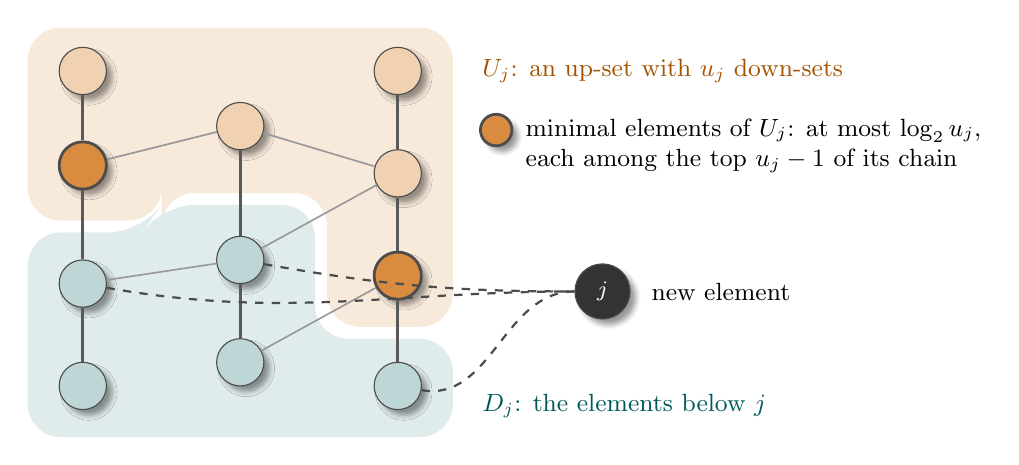
\begin{tikzpicture}[
  v/.style={circle,draw=black!70,minimum size=6mm,inner sep=0pt,font=\footnotesize,blur shadow},
  d/.style={v,fill=cD!25},
  u/.style={v,fill=cU!30},
  m/.style={v,fill=cU!75,line width=1pt},
  n/.style={v,fill=black!80,text=white,minimum size=7mm}]
\fill[cU!14,rounded corners=12pt] (-0.7,2.1) -- (1.0,2.1) -- (1.0,2.45) -- (3.1,2.45) -- (3.1,0.75) -- (4.7,0.75) -- (4.7,4.55) -- (-0.7,4.55) -- cycle;
\fill[cD!12,rounded corners=12pt] (-0.7,-0.65) -- (4.7,-0.65) -- (4.7,0.6) -- (2.95,0.6) -- (2.95,2.3) -- (1.0,2.3) -- (0.75,1.95) -- (-0.7,1.95) -- cycle;
\node[d] (a1) at (0,0) {}; \node[d] (a2) at (0,1.3) {}; \node[m] (a3) at (0,2.8) {}; \node[u] (a4) at (0,4.0) {};
\node[d] (b1) at (2,0.3) {}; \node[d] (b2) at (2,1.6) {}; \node[u] (b3) at (2,3.3) {};
\node[d] (c1) at (4,0) {}; \node[m] (c2) at (4,1.4) {}; \node[u] (c3) at (4,2.7) {}; \node[u] (c4) at (4,4.0) {};
\draw[line width=1pt,black!65] (a1)--(a2)--(a3)--(a4) (b1)--(b2)--(b3) (c1)--(c2)--(c3)--(c4);
\draw[line width=0.6pt,black!40] (a2)--(b2) (b1)--(c2) (a3)--(b3) (c3)--(b3) (b2)--(c3);
\node[n] (j) at (6.6,1.2) {$j$};
\foreach \x in {a2,b2,c1}{\draw[line width=0.8pt,black!70,dashed] (\x) to[out=-10,in=180] (j);}
\node[font=\small,cU!80!black,anchor=west] at (4.95,4.0) {$U_j$: an up-set with $u_j$ down-sets};
\node[font=\small,cD,anchor=west] at (4.95,-0.25) {$D_j$: the elements below $j$};
\node[m,minimum size=4mm] at (5.25,3.25) {};
\node[font=\small,anchor=west,align=left] at (5.5,3.05) {minimal elements of $U_j$: at most $\log_2 u_j$,\\each among the top $u_j-1$ of its chain};
\node[font=\small,anchor=west] at (7.1,1.2) {new element};
\end{tikzpicture}
\end{document}
